\documentclass[tikz,border=2pt]{standalone}
\usepackage{amsmath,amssymb}
\usetikzlibrary{arrows.meta}
\begin{document}
% (T,S) = (3,8) policy, demands 2,3,1,4,0,3,2,5,1,2 in periods 1..10, P_1 = 8.
% Each period shows the start position P_k (left half) and the end position P_k' (right half).
% Orders are placed only at the starts of periods 3, 6, 9 (k a multiple of T = 3), each lifting the
% position to S = 8: Q_3 = 5, Q_6 = 5, Q_9 = 10; between reviews the position may fall below zero (P_8' = -2).
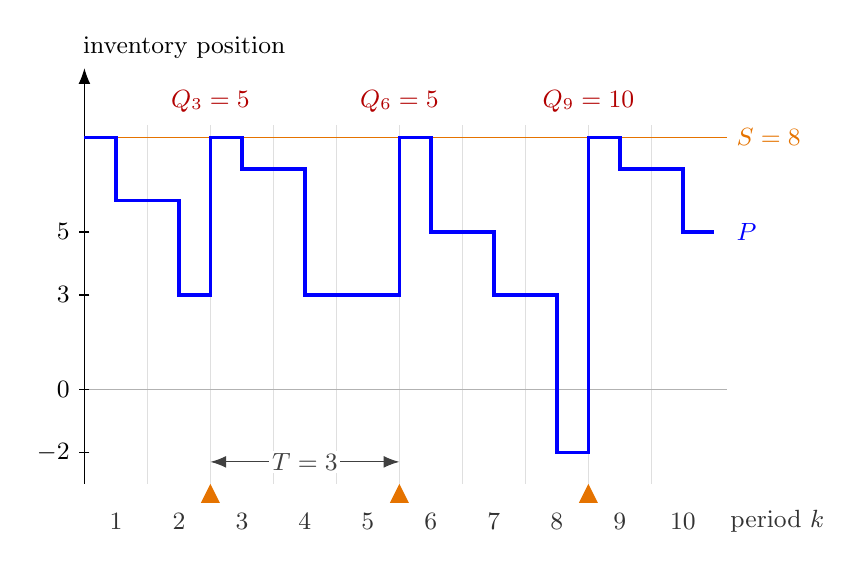
\begin{tikzpicture}[font=\small, >={Latex[length=2mm]}, x=0.8cm, y=0.4cm]
  \foreach \k in {1,...,9} {\draw[gray!25] (\k,-3) -- (\k,8.4);}
  \draw[gray!60] (0,0) -- (10.2,0);
  \draw[->] (0,-3) -- (0,10.2) node[anchor=south west, xshift=-4pt] {inventory position};
  \foreach \v in {-2,0,3,5} {\draw (0.08,\v) -- (-0.08,\v) node[left] {$\v$};}
  \foreach \k in {1,...,10} {\node[gray!40!black] at (\k-0.5,-4.2) {$\k$};}
  \node[gray!40!black, anchor=west] at (10.1,-4.2) {period $k$};
  % review epochs
  \foreach \x in {2,5,8} {\fill[orange!90!black] (\x,-3) -- (\x-0.15,-3.6) -- (\x+0.15,-3.6) -- cycle;}
  \draw[orange!90!black, thin] (0,8) -- (10.2,8) node[right] {$S=8$};
  \draw[gray!50!black, <->] (2,-2.3) -- (5,-2.3) node[midway, fill=white, inner sep=1pt] {$T=3$};
  % position path
  \draw[blue, very thick] (0,8) -- (0.5,8) -- (0.5,6) -- (1,6) -- (1.5,6) -- (1.5,3) -- (2,3) -- (2,8) -- (2.5,8) -- (2.5,7) -- (3,7) -- (3.5,7) -- (3.5,3) -- (4,3) -- (4.5,3) -- (5,3) -- (5,8) -- (5.5,8) -- (5.5,5) -- (6,5) -- (6.5,5) -- (6.5,3) -- (7,3) -- (7.5,3) -- (7.5,-2) -- (8,-2) -- (8,8) -- (8.5,8) -- (8.5,7) -- (9,7) -- (9.5,7) -- (9.5,5) -- (10,5);
  \node[blue, anchor=west] at (10.2,5) {$P$};
  % order sizes at the reviews
  \foreach \x/\k/\q in {2/3/5,5/6/5,8/9/10} {\node[red!70!black, anchor=south] at (\x,8.5) {$Q_{\k}=\q$};}
\end{tikzpicture}
\end{document}
